% \documentclass[compacto,10pt]{aleph-notas}
\documentclass[compacto,10pt,comentarios]{aleph-notas}

% -- Paquetes adicionales
\usepackage{enumitem}
\usepackage{aleph-comandos}
\usepackage{parskip}
\usepackage{graphicx}
\usepackage{xfrac}
\usepackage{tikz}
\usepackage{etoolbox}
\usepackage[framemethod=tikz]{mdframed}
\DeclareFontFamily{U}{skulls}{}
\DeclareFontShape{U}{skulls}{m}{n}{ <-> skull }{}
\newcommand{\skull}{\text{\usefont{U}{skulls}{m}{n}\symbol{'101}}}
\def \ds{\displaystyle}
\def \dfx{\dfrac{d}{dx}}
\DeclareMathOperator{\arccot}{arccot}
\DeclareMathOperator{\arcsec}{arcsec}
\DeclareMathOperator{\arccsc}{arccsc}

% -- Datos del libro
\institucion{Southwestern College}
\asignatura{MATH 251: Calculus II}
\tema{Trigonometric Functions and Their Inverses}
\autor{Jesús Pérez Cuarenta}
% \fecha{Fall 2024}

%% --> Logos de las guias
\logouno[4.5cm]{../Images/swc_logo}
\definecolor{colordef}{cmyk}{0.81, 0.62, 0.00, 0.22}

%% -- Solucion para alumnos
% \AtBeginEnvironment{proof}{\color{white}}

\begin{document}

\encabezado

\section*{Trigonometric Functions and Their Inverses}
\begin{mdframed}
    \center Learning Objectives \\
    \begin{itemize}
        \item Find the exact value of expressions involving the inverse sine, cosine, and tangent functions.
        \item Define the inverse secant, cosecant, and cotangent functions. 
        \item Use properties of inverse functions to find exact values of composite functions.
        \item Differentiate inverse trigonometric functions.
        \item Solve integrals involving inverse trigonometric functions.
    \end{itemize}
\end{mdframed}

We begin with the sine function, $f(x) = \sin(x)$. Recall that the sine function is periodic with period $2\pi$. Since we require a one-to-one correspondence for inverse functions to exist, we make a choice to restrict $\sin(x)$ to the interval $[-\frac{\pi}{2}, \frac{\pi}{2}]$.

\begin{figure}[h!]
    \centering
        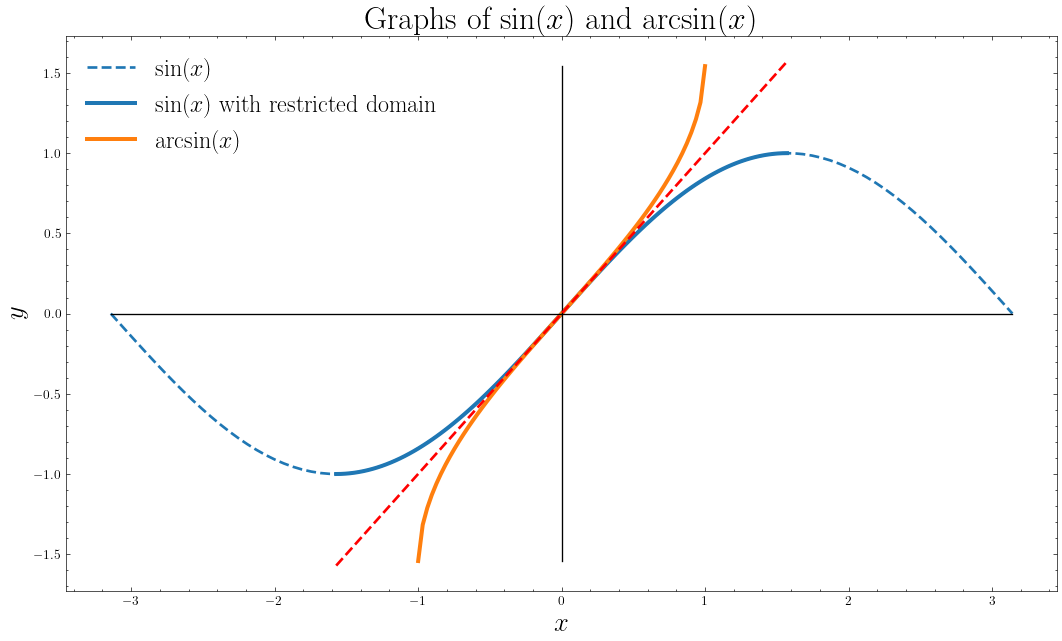
\includegraphics[width=1\linewidth]{../Images/07_05_sine.png}
\end{figure}

We will make use of the notation
$$
    f^{-1}(x) = \sin^{-1}(x) = \arcsin(x)
$$
to denote the inverse sine function.

%%%%%%%%%%%%%%%%%%%%%%%%%%%%%%%%%%%%%%%%%%%%%%%%%%%%
%% Examples
%%%%%%%%%%%%%%%%%%%%%%%%%%%%%%%%%%%%%%%%%%%%%%%%%%%%
\begin{ejer}
    Find the exact value of the following
    \begin{enumerate}
        \item $\sin^{-1}\left( \frac{\sqrt{3}}{2} \right)$
        \item $\arcsin(1)$
        \item $\sin^{-1} \left( \sin \left( \frac{1}{2} \right) \right)$
        \item $\arcsin(\sin(120^{\circ}))$
        \item $\arcsin \left( \sin \left( \frac{3\pi}{5} \right) \right)$
    \end{enumerate}
\end{ejer}
\begin{proof}[Solution]
    We have
    \begin{enumerate}
        \item 
        \begin{align*}
            \theta & = \sin^{-1}\left( \frac{\sqrt{3}}{2} \right) \\
                % \implies \sin(\theta) & = \sin \left( \sin^{-1}\left( \frac{\sqrt{3}}{2} \right) \right) \\
                \implies \sin(\theta) & = \frac{\sqrt{3}}{2} \\
                \implies \theta & = \frac{\pi}{3}.
        \end{align*}
        \item 
        \begin{align*}
            \theta & = \arcsin(1) \\
            \implies \sin(\theta) & = 1 \\
            \implies \theta & = \frac{\pi}{2}.
        \end{align*}
        \item 
        $$
            \sin^{-1} \left( \sin \left( \frac{1}{2} \right) \right) = \frac{1}{2}.
        $$
        \item $\skull$
        $$
            \arcsin(\sin(120^{\circ})) = 60 ^{\circ}.
        $$
        \item $\skull$
        $$
            \arcsin \left( \sin \left( \frac{3\pi}{5} \right) \right) = \frac{2\pi}{5}.
        $$
    \end{enumerate}
\end{proof}

We can follow a similar argument for the cosine function (try it!). Afterwards, you can convince yourself that a good interval to subset $\cos(x)$ is over $[0, \pi]$.
\begin{defi}[\textbf{Inverse Sine and Cosine}]
    We take $y = \sin^{-1}(x)$ as the values of $y$ such that $x = \sin{y}$, where $-\frac{\pi}{2} \leq y \leq \frac{\pi}{2}$. \\
    We take $y = \cos^{-1}(x)$ as the values of $y$ such that $x = \cos{y}$, where $0 \leq y \leq \pi$. \\
    The domain of both $\sin^{-1}(x)$ and $\cos^{-1}(x)$ is $\{ x: -1 \leq x \leq 1 \}$.
\end{defi}

\begin{ejer}
    Find the exact value of the following
    \begin{enumerate}
        \item $\cos^{-1}\left( - \frac{\sqrt{2}}{2} \right)$
        \item $\arccos(0)$
        \item $\cos^{-1} \left( \cos \left( - \frac{2\pi}{3} \right) \right)$
    \end{enumerate}
\end{ejer}
\begin{proof}[Solution]
    We have
    \begin{enumerate}
        \item
        \begin{align*}
            \theta & = \cos^{-1}\left( - \frac{\sqrt{2}}{2} \right) \\
            \implies \cos(\theta) & = - \frac{\sqrt{2}}{2} \\
            \implies \theta & = \frac{3\pi}{4} .
        \end{align*}
        \item
        \begin{align*}
            \theta & = \arccos(0) \\
            \implies \cos(\theta) & = 0 \\
            \implies \theta & = \frac{\pi}{2} .
        \end{align*}
        \item $\skull$
        $$
        \cos^{-1} \left( \cos \left( - \frac{2\pi}{3} \right) \right) = \frac{2\pi}{3}.
        $$
    \end{enumerate}
\end{proof}

The remaining inverse trigonometric functions are defined as follows.
\begin{defi}
    We take $y = \tan^{-1}(x)$ as the values of $y$ such that $x = \tan(y)$, where $-\frac{\pi}{2} \leq y \leq \frac{\pi}{2}$. \\

    We take $y = \cot^{-1}(x)$ as the values of $y$ such that $x = \cot(y)$, where $0 \leq y \leq \pi$. \\

    The domain of both $\tan^{-1}(x)$ and $\cot^{-1}(x)$ is $\{ x: -\inf < x < \inf \}$. \\

    We take $y = \sec^{-1}(x)$ as the values of $y$ such that $x = \sec{y}$, where $0 \leq y \leq \pi$, with $y \neq \frac{\pi}{2}$. \\

    We take $y = \csc^{-1}(x)$ as the values of $y$ such that $x = \csc(y)$, where $-\frac{\pi}{2} \leq y \leq \frac{\pi}{2}$, with $y \neq 0$. \\

    The domain of both $\sec^{-1}(x)$ and $\csc^{-1}(x)$ is $\{x: |x| \geq 1 \}$.
\end{defi}

Here is a useful summary.
\begin{table}[h!]
    \centering
    \renewcommand{\arraystretch}{1.5}  % Increase row height
    \begin{tabular}{|c|c|c|}
    \hline
    \textbf{Function} & \textbf{Domain} & \textbf{Range} \\
    \hline
    $y = \sin^{-1} x$   & $-1 \leq x \leq 1$ & $\frac{-\pi}{2} \leq y \leq \frac{\pi}{2}$ \\
    \hline
    $y = \cos^{-1} x$  & $-1 \leq x \leq 1$ & $0 \leq y \leq \pi$ \\
    \hline
    $y = \tan^{-1} x$ & $x \in \mathbb{R}$ & $\frac{-\pi}{2} < y < \frac{\pi}{2}$ \\
    \hline
    $y = \cot^{-1} x$  & $x \in \mathbb{R}$ & $0 < y < \pi$ \\
    \hline
    $y = \csc^{-1} x$   & $x \leq -1 \; \text{or} \; x \geq 1$ & $\frac{-\pi}{2} \leq y \leq \frac{\pi}{2}, \; y \neq 0$ \\
    \hline
    $y = \sec^{-1} x$  & $x \leq -1 \; \text{or} \; x \geq 1$ & $0 \leq y \leq \pi, \; y \neq \frac{\pi}{2}$ \\
    \hline
    \end{tabular}
\end{table}

\begin{ejer}
    Find the exact value of the following.
    \begin{enumerate}
        \item $\arctan\left( \frac{\sqrt{3}}{3} \right)$
        \item $\arctan(1)$
        \item $\cot^{-1}\left( \frac{\sqrt{3}}{3} \right)$
        \item $\csc^{-1} \left( \sqrt{2} \right)$
    \end{enumerate}
\end{ejer}
\begin{proof}[Solution]
    We have
    \begin{enumerate}
        \item 
        \begin{align*}
            \theta & = \arctan \left( \frac{\sqrt{3}}{3} \right) \\
            \implies \tan{\theta} & = \frac{\sqrt{3}}{3} \\
            \implies \theta & = \frac{\pi}{6} .
        \end{align*}
        \item 
        \begin{align*}
            \theta & = \arctan \left( 1 \right) \\
            \implies \tan{\theta} & = 1 \\
            \implies \theta & = \frac{\pi}{4} .
        \end{align*}
        \item 
        \begin{align*}
            \theta & = \cot^{-1} \left( \frac{\sqrt{3}}{3} \right) \\
            \implies \cot{\theta} & = \frac{\sqrt{3}}{3} \\
            \implies \theta & = \frac{\pi}{3} .
        \end{align*}
        \item 
        \begin{align*}
            \theta & = \csc^{-1} \left( \sqrt{2} \right) \\
            \implies \csc(\theta) & = \sqrt{2} \\
            \implies \theta & = \frac{\pi}{4} .
        \end{align*}
    \end{enumerate}
\end{proof}

\begin{ejer}
    Suppose $\theta = \sin^{-1} \left( \frac{2}{5} \right)$. Find $\cos(\theta)$ and $\tan(\theta)$.
\end{ejer}
\begin{proof}[Solution]
    We have
    $$
    \sin(\theta) = \frac{2}{5}
    $$
    which has the following geometric representation.
    \begin{center}
        \begin{tikzpicture}
            \coordinate (a) at (0, 0);
            \coordinate (b) at (4, 0);
            \coordinate (c) at (4, 2);
            \draw (a) -- (b)node[midway, below]{$x = \sqrt{21}$} -- (c)node[midway, right]{2} -- (a)node[midway, left, above]{5};
            \draw (1, 0) arc (0:25:1)node[midway, right]{$\theta$};
        \end{tikzpicture}
    \end{center}
    Note that $x$ is obtained via the Pythagorean theorem. Thus,
    \begin{align*}
        \cos(\theta) & = \frac{\sqrt{21}}{5}, \\
        \tan(\theta) & = \frac{2}{\sqrt{21}} = \frac{2\sqrt{21}}{21} .
    \end{align*}
\end{proof}

\begin{ejer}
    Find an alternative form for $\cot\left( \cos^{-1} \left( \frac{x}{4} \right) \right)$.
\end{ejer}
\begin{proof}[Solution]
    Let $\theta = \cos^{-1} \left( \frac{x}{4} \right)$. It follows that
    \begin{align*}
        \cos(\theta) & = \frac{x}{4}
    \end{align*}
    which has the following geometric representation.
    \begin{center}
        \begin{tikzpicture}
            \coordinate (a) at (0, 0);
            \coordinate (b) at (4, 0);
            \coordinate (c) at (4, 2);
            \draw (a) -- (b)node[midway, below]{$x$} -- (c)node[midway, right]{$\sqrt{16 - x^2}$} -- (a)node[midway, left, above]{4};
            \draw (1, 0) arc (0:25:1)node[midway, right]{$\theta$};
        \end{tikzpicture}
    \end{center}
    It follows that
    $$
    \cot \left( \cos^{-1} \left( \frac{x}{4} \right) \right) = \frac{x}{\sqrt{16 - x^2}}.
    $$
\end{proof}

\begin{ejer}
    Derive the formula for $\frac{d}{dx} \arctan(x)$.
\end{ejer}
\begin{proof}[Solution]
    Let $\theta = \arctan(x)$. Now
    \begin{align*}
        \tan\left(\theta\right) & = \frac{x}{1}
    \end{align*}
    has the following geometric representation.
    \begin{center}
        \begin{tikzpicture}
            \coordinate (a) at (0, 0);
            \coordinate (b) at (4, 0);
            \coordinate (c) at (4, 2);
            \draw (a) -- (b)node[midway, below]{$1$} -- (c)node[midway, right]{$x$} -- (a)node[midway, left, above]{$\sqrt{1 + x^2} \quad \quad $};
            \draw (1, 0) arc (0:25:1)node[midway, right]{$\theta$};
        \end{tikzpicture}
    \end{center}
    We differentiate the equation $\tan(\theta) = x$ with respect to $x$,
    \begin{align*}
    \frac{d}{dx} \tan(\theta) & = \frac{d}{dx} x \\
    \implies \sec^{2}(\theta) \frac{d\theta}{dx} & = 1 \\
    \implies \frac{d\theta}{dx} & = \cos^{2}(\theta) \\
    \implies \frac{d\theta}{dx} & = \frac{1}{1+x^{2}}.
    \end{align*}
    Therefore,
    $$
    \frac{d}{dx} \arctan(x) = \frac{1}{1 + x^2}.
    $$
\end{proof}

\begin{ejer}
    Derive the formula for $\frac{d}{dx} \arcsin(x)$.
\end{ejer}
\begin{proof}[Solution]
    Let $\theta = \arcsin(x)$. Now
    \begin{align*}
        \sin\left(\theta\right) & = \frac{x}{1}
    \end{align*}
    has the following geometric representation.
    \begin{center}
        \begin{tikzpicture}
            \coordinate (a) at (0, 0);
            \coordinate (b) at (4, 0);
            \coordinate (c) at (4, 2);
            \draw (a) -- (b)node[midway, below]{$\sqrt{1 - x^2}$} -- (c)node[midway, right]{$x$} -- (a)node[midway, left, above]{$1$};
            \draw (1, 0) arc (0:25:1)node[midway, right]{$\theta$};
        \end{tikzpicture}
    \end{center}
    We differentiate the equation $\sin(\theta) = x$ with respect to $x$,
    \begin{align*}
    \frac{d}{dx} \sin(\theta) & = \frac{d}{dx} x \\
    \implies \cos(\theta) \frac{d\theta}{dx} & = 1 \\
    \implies \frac{d\theta}{dx} & = \sec{\theta} \\
    \implies \frac{d\theta}{dx} & = \frac{1}{\sqrt{1-x^2}} ~ .
    \end{align*}
    Therefore,
    $$
    \frac{d}{dx} \arcsin(x) = \frac{1}{\sqrt{1-x^2}} ~ .
    $$
\end{proof}

In general, we have the following derivatives.
\begin{defi}[Inverse Trigonometric Function Derivatives]
    Let $u$ be a differentiable function in terms of $x$. Then
    \begin{align*}
        \frac{d}{dx} \arcsin(u) & = \frac{u'}{\sqrt{1 - u^2}} \\
        \frac{d}{dx} \arccos(u) & = -\frac{u'}{\sqrt{1 - u^2}} \\
        \frac{d}{dx} \arctan(u) & = \frac{u'}{1 + u^2} \\
        \frac{d}{dx} \arccot(u) & = -\frac{u'}{1 + u^2} \\
        \frac{d}{dx} \arcsec(u) & = \frac{u'}{|u| \sqrt{u^2 - 1}} \\
        \frac{d}{dx} \arccsc(u) & = -\frac{u'}{|u| \sqrt{u^2 - 1}}
    \end{align*}
\end{defi}

\begin{ejer}
    Find the derivative for each function. Simplify if possible.
    \begin{enumerate}
        \item $h(t) = 4\arctan(2t)$
        \item $p(x) = 16 \arcsin\left( \frac{x}{4} \right)$
        \item $f(x) = 2x\arccos(x) - 2 \sqrt{1 - x^2}$
    \end{enumerate}
\end{ejer}
\begin{proof}[Solution]
    We have
    \begin{enumerate}
        \item Let $u(t) = 2t$, then $u'(t) = 2$. Hence,
        \begin{align*}
            \frac{d}{dt} h(t) & = \frac{d}{dt} \left( 4 \arctan(2t) \right) \\
            & = \left( 4 \right) \left( \frac{1}{1 + (2t)^{2}} \right) \left( 2 \right) \\
            & = \frac{8}{1 + 4t^2} ~ .
        \end{align*}
        \item Let $u(x) = \frac{x}{4}$, then $u'(x) = \frac{1}{4}$. Hence,
        \begin{align*}
            \frac{d}{dx} p(x) & = \frac{d}{dx} \left( 16 \arcsin\left( \frac{x}{4} \right) \right) \\
            & = \left( 16 \right) \left(  \frac{1}{\sqrt{1 - \left( \frac{x}{4} \right)^{2} }} \right) \left( \frac{1}{4} \right) \\
            & = \frac{16}{\sqrt{16 - x^2}} ~ .
        \end{align*}
        \item Here we apply the product rule
        \begin{align*}
            \frac{d}{dx} f(x) & = \frac{d}{dx} \left( 2x\arccos(x) - 2 \sqrt{1 - x^2} \right) \\
            & = 2 \left(  -\frac{x}{\sqrt{1 - x^2}}  + \arccos(x) \right) + \frac{2x}{\sqrt{1-x^2}} \\
            & = 2 \arccos(x) ~ .
        \end{align*}
    \end{enumerate}
\end{proof}

\begin{ejer}
    Consider the equation $x^2 + x \arctan(y) = y - 1$ at the point $\left( -\frac{\pi}{4}, 1 \right)$. Find (i) the slope and (ii) the equation of the tangent line at the given point.
\end{ejer}
\begin{proof}[Solution]
    First we find the slope at the point via implicit differentiation
    \begin{align*}
        \frac{d}{dx} \left( x^2 + x \arctan(y) \right) & = \frac{d}{dx} \left( y - 1 \right) \\
        \implies 2x + \frac{x y'}{1 + y^2} + \arctan(y) & = y' \\
        \implies \left(1 - \frac{x}{1+y^2} \right) y' & =  2x + \arctan(y) \\
        \implies y' & = \left(1 - \frac{x}{1+y^2} \right)^{-1} \left( 2x + \arctan(y) \right) ~ .
    \end{align*}
    We apply the given coordinates
    \begin{align*}
        y' & = \left( 1 + \frac{\pi}{8} \right)^{-1} \left( -\frac{\pi}{2} + \arctan(1) \right) \\
        & = \left( \frac{8}{8 + \pi} \right) \left( - \frac{\pi}{4} \right) \\
        & = -\frac{2\pi}{8 + \pi} ~ . 
    \end{align*}
    From previous mathematics courses, we know that the equation for a line given the slope $m$ and point $(x_{1}, y_{1})$ is
    $$
    y - y_1 = m (x - x_{1}).
    $$
    Hence, the equation of the line tangent to $x^{2} + x\arctan(y) = y - 1$ at $(-\frac{\pi}{4}, 1)$ is
    $$
    y = -\frac{2\pi}{8 + \pi} \left( x + \frac{\pi}{4} \right) + 1 ~ .
    $$
\end{proof}

In addition to derivatives, we now pay attention to integrals.
\begin{defi}
Let $a \in \mathbb{R}$ with $a \neq 0$. Then
\begin{align*}
    \int \frac{du}{\sqrt{a^2 - u^{2}}} & = \arcsin\left( \frac{u}{a} \right) + C \\
    \int \frac{du}{a^{2} + u^{2}} & = \frac{1}{a} \arctan \left( \frac{u}{a} \right) + C \\
    \int \frac{du}{u \sqrt{u^{2} - a^{2}}} & = \frac{1}{a} \arcsec\left( \frac{|u|}{a} \right) + C
\end{align*}
    for some $C \in \mathbb{R}$.
\end{defi}

\begin{ejer}
    Evaluate each integral.
    \begin{enumerate}
        \item
        $$
            \int \frac{2}{\sqrt{16 - 9x^2}} ~ dx
        $$
        \item
        $$
            \int \frac{{\rm e}^{x}}{4 + {\rm e}^{2x}} ~ dx
        $$
        \item
        $$
            \int \frac{5}{3x\sqrt{x - 4}} ~ dx
        $$
        \item
        $$
            \int \frac{2}{\sqrt{-x^2-4x}} ~ dx
        $$
        \item 
        $$
            \int_{0}^{\sfrac{1}{2}} \frac{\arccos(x)}{\sqrt{1 - x^2}} ~ dx
        $$
    \end{enumerate}
\end{ejer}
\begin{proof}[Solution]
    We have
    \begin{enumerate}
        \item Let $a = 4$ and $ u = 3x$, then
        $$
        \int \frac{2}{\sqrt{16 - 9x^2}} ~ dx = \frac{2}{3} \int \frac{3~ dx}{\sqrt{(4)^2 - (3x)^2}} = \frac{2}{3} \arcsin\left( \frac{3x}{4} \right) + C
        $$
        \item With $u = {\rm e}^{x}$, we get
        $$
        \int \frac{{\rm e}^{x}}{4 + {\rm e}^{2x}} ~ dx = \int \frac{du}{(2)^2 + (u)^2} = \frac{1}{2} \arctan\left( \frac{{\rm e}^{x}}{2} \right) + C
        $$
        \item $\skull$
        $$
        \int \frac{5}{3x\sqrt{x - 4}} ~ dx = \frac{10}{3} \int \frac{du}{4 + u^2} = \frac{5}{3} \arctan \left( \frac{\sqrt{x-4}}{2} \right) + C
        $$
        \item $\skull$
        $$
            \int \frac{2}{\sqrt{-x^2-4x}} ~ dx = 2 \int \frac{1}{\sqrt{4 - (x+2)^2}} ~ dx = 2 \arcsin \left( \frac{x+2}{2} \right) + C
        $$
        \item Let $u = \arccos(x)$, then $du = -\frac{1}{\sqrt{1 - x^2}} ~ dx$ so that
        $$
            \int \frac{\arccos(x)}{\sqrt{1 - x^2}} ~ dx = \int -u~du = -\frac{1}{2} \left( \arccos(x) \right)^2 + C.
        $$
        Applying the bounds,
        \begin{align*}
            \int_{0}^{\sfrac{1}{2}} \frac{\arccos(x)}{\sqrt{1 - x^2}} ~ dx & = \left. -\frac{1}{2} \left( \arccos(x) \right)^2 \right\rvert_{0}^{\sfrac{1}{2}} \\
            & = -\frac{1}{2} \left( \left( \arccos \left( \frac{1}{2} \right) \right)^{2} - \left( \arccos \left( 0 \right) \right)^{2} \right) \\
            & = -\frac{1}{2} \left( \frac{\pi^2}{9} - \frac{\pi^2}{4} \right) \\
            & = -\frac{1}{2} \left( \frac{\pi^2}{9} - \frac{\pi^2}{4} \right) \\
            & = \frac{5\pi^2}{72} ~ .
        \end{align*}
    \end{enumerate}
\end{proof}

To end the section, kindly acknowledge the difference between
$$
\int \frac{x}{x^2 + 9}~dx
$$
and
$$
\int \frac{1}{x^2 + 9}~dx.
$$
\end{document}